\chapter{Theoretische Grundlagen}
\section{Der Cubesat Designstandard}
	\subsection{Historische Entwicklung}
Die Fortschritte in der modernen Technologie unterstützen die Entwicklung der miniaturisierten Satelliten. Durch den Fokus der wissenschaftlichen Gemeinschaft auf Nano- und Picosatelliten sind die CubeSats zu einem wichtigen Teil der Kategorie geworden. Mit der Einführung des CubeSat-Konzepts 1998, mit der die Standardisierung von Masse und Größe von Satelliten inher ging, stieg die Zugänglichkeit des Weltraumes. Des Weiteren zeichnen sie sich durch ihre Modularität, leistungsstarken und kommerziell erhältlichen Satellitenkomponenten (commercial off-the-shelf) und ihren schnellen Entwicklungszyklen aus. Infolge der Standardisierung des CubeSats wurde das Startsystem Poly-Picosatellit Orbit Deployer (P-POD) entwickelt um eine kostengünstige Lösung für die Entwicklung und den sicheren Start bereitzustellen [Literatur]. 2003 wurde die  erste CubeSat Mission durchgeführt. Seitdem werden sie mit stark zunehmender Häufigkeit eingesetzt. Dies wird in \abb{fig:NanosatsTypes} veranschaulicht.
			\begin{figure}[h]
				\centering
					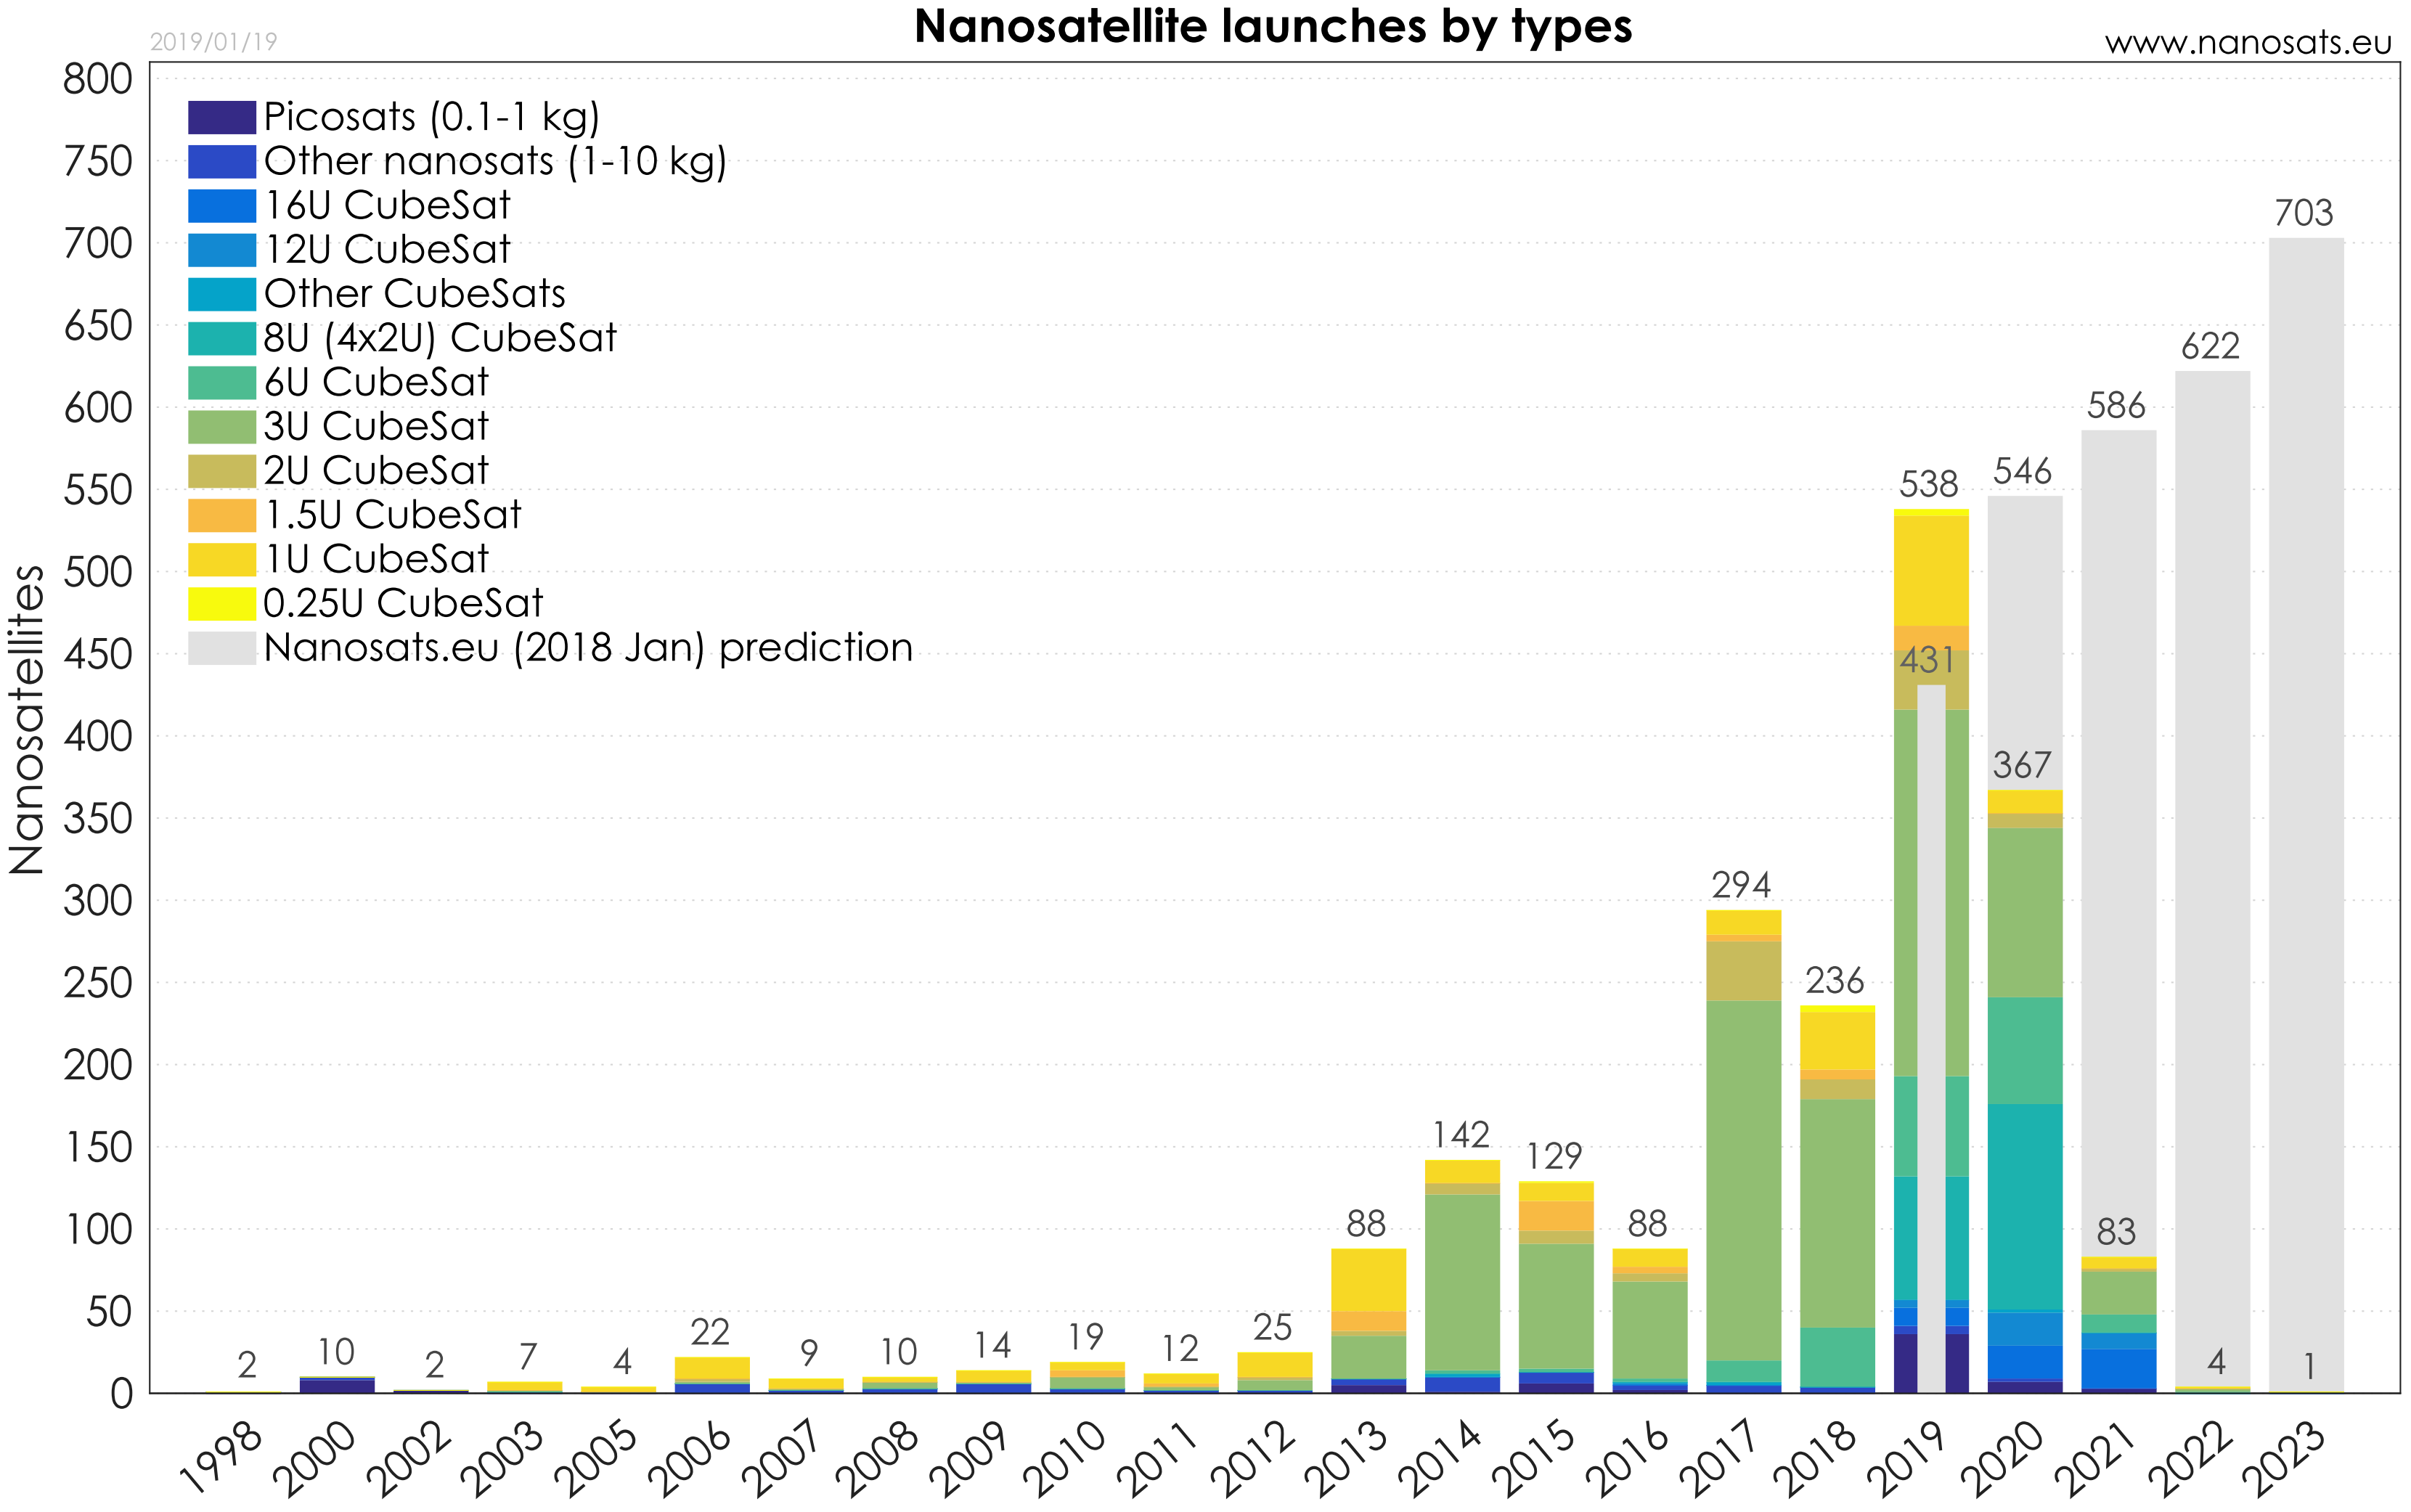
\includegraphics[width=0.80\textwidth]{Nanosats_years_types_2019-01-19_01}
				\caption{Überblick über Nanosatelliten.Missionen von 1998 bis 2023}
				\label{fig:NanosatsTypes}
			\end{figure}

	\newpage
	\subsection{Gestaltungsrichtlinien}
Für die Gestaltung von CubeSats gelten eine Reihe von Richtlinien. Als kleinste Einheit (1U) wird ein Würfel mit einer Kantenlänge von 10cm und einer zulässigen Masse von maximal 1,33 kg vorgegeben. Für größere Volumen und Massen können mehrere Einheiten von CubeSats verbunden werden. Satelliten mit 1U, 1.5U, 2U, oder 3U können von dem einheitlichen Startmechanismus (P-Pod) in die Erdumlaufbahn ausgelassen werden. Die Kosten von CubeSat Missionen können gering gehalten werden, indem diese als sekundäre Nutzlast bei Raketenstarts mitfliegen. Für größere Satelliten (6U, 12U, 27U) werden andere Startmechanismen benötigt. Die zugelassene Masse wird auf 2 kg/U angehoben. Weitere Vorschriften gelten für die Folgenden Kriterien:
		\begin{itemize}
			\item \textit{Materialien:} 	\\ Alle bei der Konstruktion verwendeten Materialien müssen den Richtlinien der Air Force Space Command Manual \textbf{[AFSPCMAN 91-710 Volume 3]} entsprechen. Außerdem darf der Masseverlust des Satelliten maximal 1\% betragen.
			\item \textit{Energiespeicher:} \\ Der chemische Energiespeicher darf eine Größe von 100 Wh nicht überschreiten. 
			\item \textit{Aktivierungszeitpunkt:} \\ Während der CubeSat im P-POD verstaut ist müssen alle Systeme ausgeschaltet bleiben. Beim Verlassen der Trägerrakete wird der Satellit aktiviert. Erst 30 Minuten später dürfen Bauteile (z.B. Solarpanele, Antennen, etc...) ausgefahren werden. Bevor die ersten Signale generiert oder gesendet werden müssen mindestens 45 Minuten vergangen sein. 
		\end{itemize}
%Allgemein gelten noch weitere Vorschriften für die verwendeten  Materialien, Kommunikationsfähigkeit, gespeicherte Energie und Aktivierungszeitpunkt der Systeme nach Einsatz in die Umlaufbahn. 
Falls ein Entwurf nicht den Vorschriften entspricht, kann bei dem Betreiber der Trägerrakete eine Sondergenehmigung angefragt werden. Nach einer Reihe von Tests entscheidet dieser ob er die Abweichungen akzeptiert, Änderungen vorgenommen werden müssen, oder ein anderer Anbieter gefunden werden muss. 

	\section{Cubesat Subsysteme}
	%hier Hauptsächlich das Fazit von max kompakt darstellen und refernzieren
		\subsection{Antrieb}
Eines der wichtigsten Subsysteme für Active Debris Removal (ADR) Missionen mit einem CubeSat ist der Antrieb. Er wird für Lageregelung und das Deorbiting des Zielobjekts benötigt.  Um Lageregelung und Rendezvous-Manöver durchführen zu können müssen sehr präzise Triebwerke gewählt werden. 
Für CubeSats stehen nur wenige ausgereifte und erprobte Triebwerke zur Verfügung [Literatur].  Die Miniaturisierung bestehender Technologien stellt eine große Herausforderung dar. Ein hoher technology readiness level  (TRL) ist für die Auswahl besonders Entscheidend, da nur bereits erprobte Technologien für diese Mission genutzt werden sollten.
Im Wesentlichen lassen sich die Antriebsarten in chemische und elektrische Antriebe unterteilen.  Chemische Antriebe generieren im Allgemeinen einen relativ hohen Schub und werden für impulsive Manöver verwendet. Für den Betrieb muss eine vergleichbar großer Gewichtsanteil an Treibstoff einkalkuliert werden. Der spezifische Impuls ist jedoch deutlich niedriger als bei elektrischen Antrieben. Diese bieten auch ein besseres Schub-Leistungs-Verhältnis. Elektrische Antriebe sind jedoch auf eine ausreichende externe Energiequelle angewiesen. Diese wird zwangsläufig benötigt, um die getankte Masse zu beschleunigen [Literatur].
Für genaue Untersuchung und den Vergleich der verschiedenen Triebwerkstypen wird auf die [Literatur] verwiesen. Miniaturisierte Versionen von erprobten Triebwerken werden stetig weiterentwickelt und getestet. Es wurden bereits mehrere Miniaturisierte Triebwerke in CubeSatmissionen erfolgreich eingesetzt. In Zukunft sollte es eine wachsende Auswahl an geeigneten Triebwerken für CubeSatmissionen geben. 
		\subsection{Energie - EPS}
		\subsection{Guidance, navigation and control -GNC ADCS}
		\subsection{Command and data handling}
		\subsection{Kommunikation}
		\subsection{Thermik}
		Die Wärme wird im Vakuum durch Strahlungen und Wärmeleitungen übertragen. Das Wärmemanagement regelt den Bereich der zulässigen Temperaturen für die Sicherstellung einer optimalen Funktionalität und (ein/e optimales/e Weiterbestehen/Überleben/Effizienz). Durch die Massen-, Volumen- und Leistungsbeschränkungen bei miniaturisierten Satelliten, wie dem CubeSat, liegt der Fokus auf den passiven Wärmereglungstechnologien, da die Fortschritte bei der Entwicklung von miniaturisierten aktiven Wärmeregelungsmethoden begrenzt ist. Passive Technologien sind mit geringen Kosten, Volumen, Gewicht und Risiko verbunden und erfordern keine interne Eingangsleistung für die Wärmeregulierung. Thermische Beschichtungen, Wärmerohre, Sonnenschirme, Wärmebänder und Multi-Layer Insulation (MLI) sind passive Methoden für die Regulierung des thermischen Gleichgewichtes. Die aktiven Methoden, wie elektrische Widerstandsheizungen, Kühler oder kryogene Materialien, sind mit höherer Präzision und interner Eigenleistung verbunden. Die Verwendung von aktiven Systemen ist bei temperaturempfindlichen Geräten und nicht ausreichender, passiver Systeme für eine Aufrechterhaltung der Betriebstemperatur vielversprechender [Literatur NASA Sota].

		\subsection{Struktur}
		Die Strukturen werden in Primär- und Sekundärestrukturen unterteilt. Die Primärstruktur ist thermischen und dynamischen Beeinflussungen ausgesetzt, denen sie entgegenwirken muss. Des Weiteren sorgt es für Lastübertragung während des Starts und des Einsatzes. Elektromagnetische Strahlungen, Drücke und innere Wärmeleitungen sind weitere Faktoren die einen großen Einfluss auf das Gehäuse haben und deshalb mit einbezogen werden müssen. Die Begrenzungen bei der Oberfläche und bei dem Volumen sorgen für Einschränkungen. Infolgedessen sollte sie effizient ausgelegt werden. Komponenten die nur sich selbst tragen müssen, wie Sonnenkollektoren, zählen zu den Sekundärstrukturen auf die nicht näher eingegangen wird, da sie bei einem Ausfall die Integrität des Raumfahrzeugs nicht beeinträchtigt. Die Primärstrukturen werden als COTS-Strukturen und kundenspezifisch bearbeitet oder gedruckte Komponenten auf dem Markt angeboten. Generell besteht das Gehäuse aus metallischen und nichtmetallischen Materialien und wird von der Betriebsumgebung des Satelliten bestimmt [Literatur: NASA Sota].
				
	\section{RDVDO Mechanismen} das kann ausführlich sein
		\subsection{Docking Strategien}
						\textbf{Roboterarm}
						\textbf{Fangnetz}
						\textbf{Adhäsiv Docken}
						%Übersichtstabelle/Graphik: sihe die Quellen die ich am 15.05.2019 gezeigt habe
		\subsection{Bionische Materialien}
						%\textbf{Was sind Geckomaterialen}
						%\textbf{Bisher getestete Gecko-Materialien}
						%\textbf{Bisherige Erfolge}
						%\textbf{State of the Art}
						%\textbf{Problematik}